
%
% realization - architecture + implementation
%

\section{Architecture \& Implementation}
\label{chapter:architecture-implementation}

Geocluster is a Drupal 7 module that implements the Geohash-based clustering algorithm. 
 
An iterative approach was taken in order to explore ways to fulfill the various integration and extensibility requirements formulated in chapter \ref{chapter:objective-performance} and analyzed in chapter \label{chapter:analysis-drupal}. Based on the Drupal mapping stack explained in chapter \ref{chapter:drupal-mapping}, a high-level architecture for implementing the Geohash-based clustering algorithm was designed.

\subsection{Principles}

Geocluster has been implemented following a number of principles:

\begin{itemize}

\item Leverage existing APIs and \textit{hooks} when possible
\item Program object-oriented code where it makes sense
\item Implement changes to existing modules as \textit{patches} if necessary

\end{itemize}

While using APIs and object-oriented programming are familiar concepts, \textit{hooks} are a Drupal-specific concept. They basically allow modules to interact with each other in a procedural way in which many parts of the Drupal system are built.

\begin{quote}
Drupal's module system is based on the concept of "hooks". A hook is a PHP function that is named foo\_bar(), where "foo" is the name of the module (whose filename is thus foo.module) and "bar" is the name of the hook. Each hook has a defined set of parameters and a specified result type.

To extend Drupal, a module need simply implement a hook. When Drupal wishes to allow intervention from modules, it determines which modules implement a hook and calls that hook in all enabled modules that implement it.\footnote{\url{http://api.drupal.org/api/drupal/includes!module.inc/group/hooks/7}}
\end{quote}

The term \textit{patch} describes a way to submit code changes used within the Drupal and other open source communities:

\begin{quote}
Patches are pieces of code that solve an existing issue. In fact, patches describe the changes between a before and after state of either a module or core. By applying the patch the issue should no longer exist.

Patches are used to maintain control-ability over the entire Drupal project. While Drupal is distributed via the git version control system, patches are additional pieces of code that focus on a single change request and therefore are easily tested, reviewed and documented.\footnote{\url{http://drupal.org/patch}}
\end{quote}



\subsection{Architecture overview}

The parts involved in the Geocluster system are

\begin{itemize}

\item Integration of the Geohash-based hierarchical spatial index with Geofield

\item Server-side clustering implementation
  \begin{itemize}
   \item Configuration of the clustering process
   \item Implementation of the clustering algorithm
   \item Integration of the clustering process with Views
  \end{itemize}

\item Client-side Geocluster Visualization component

\end{itemize}


\begin{figure}[h]
  \begin{center}
    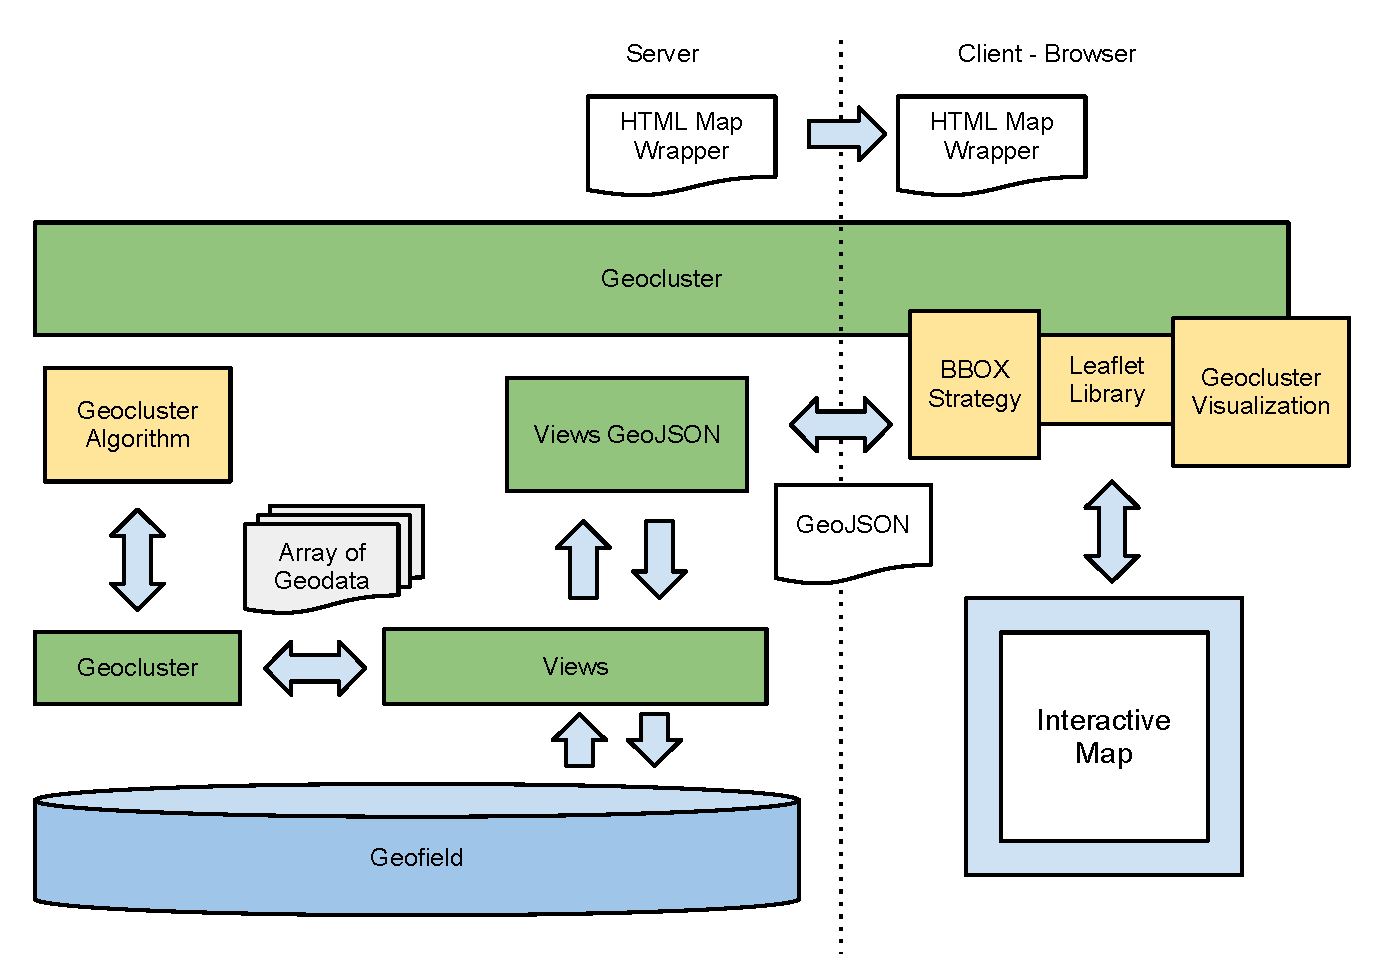
\includegraphics[width=1\textwidth]{figures/geocluster_architecture.pdf}
    \caption{Geocluster architecture overview.}
    \label{fig:geocluster-architecture}
  \end{center}
\end{figure}

Figure \ref{fig:geocluster-architecture} depicts how the Geocluster module integrates with other components of the Drupal mapping stack. The main point of integration for the Geocluster module on the server-side is the Views module. When the Views module performs a spatial query that has been configured for clustering, Geocluster will integrate the clustering algorithm into the Views execution process. The clustering task may interact with the Views module \textit{before} and \textit{after} a query has been executed. Different algorithm implementations may rely on modification of the Views query while others only need to post-process the results of a Views query. After the clustering process has been finished, the server-side execution process continues as usual. The clustered result data is rendered, for example as GeoJSON feed using the Views GeoJSON as indicated in the diagram. On the client-side, a Geocluster Visualization component is used to properly visualize clustered results. The Geocluster module therefore integrates with the Leaflet and Leaflet GeoJSON modules in order extend the Bounding-Box driven communication of clustered results between client and server.


\subsection{Integration of the Geohash-based hierarchical spatial index with Geofield}

The Drupal Field API that Geofield uses has been leveraged to spatially index locations stored by the Geofield module. The field schema for fields of the Geofield type is extended by $geocluster\_field\_schema\_alter$ to add separate columns for the Geohash indices that form the spatial index. The $geocluster\_field\_attach\_presave$ hook implementation takes care of saving the additional index information whenever a Geofield location value is saved to the database.

During the development of the Geocluster module, support for encoding location values into Geohash has been added to the geoPHP library\footnote{\url{https://github.com/phayes/geoPHP/issues/32}}. Subsequently, a patch to make use of geoPHP's Geohash support has been created for the Geofield module and committed\footnote{\url{http://drupal.org/node/1662584}}. 


\subsection{Server-clustering implementation}

The server-side clustering implementation consists of three parts: configuration of the clustering process, implementation of the clustering algorithm and integration of the clustering process with Views.

\begin{figure}[h]
  \begin{center}
    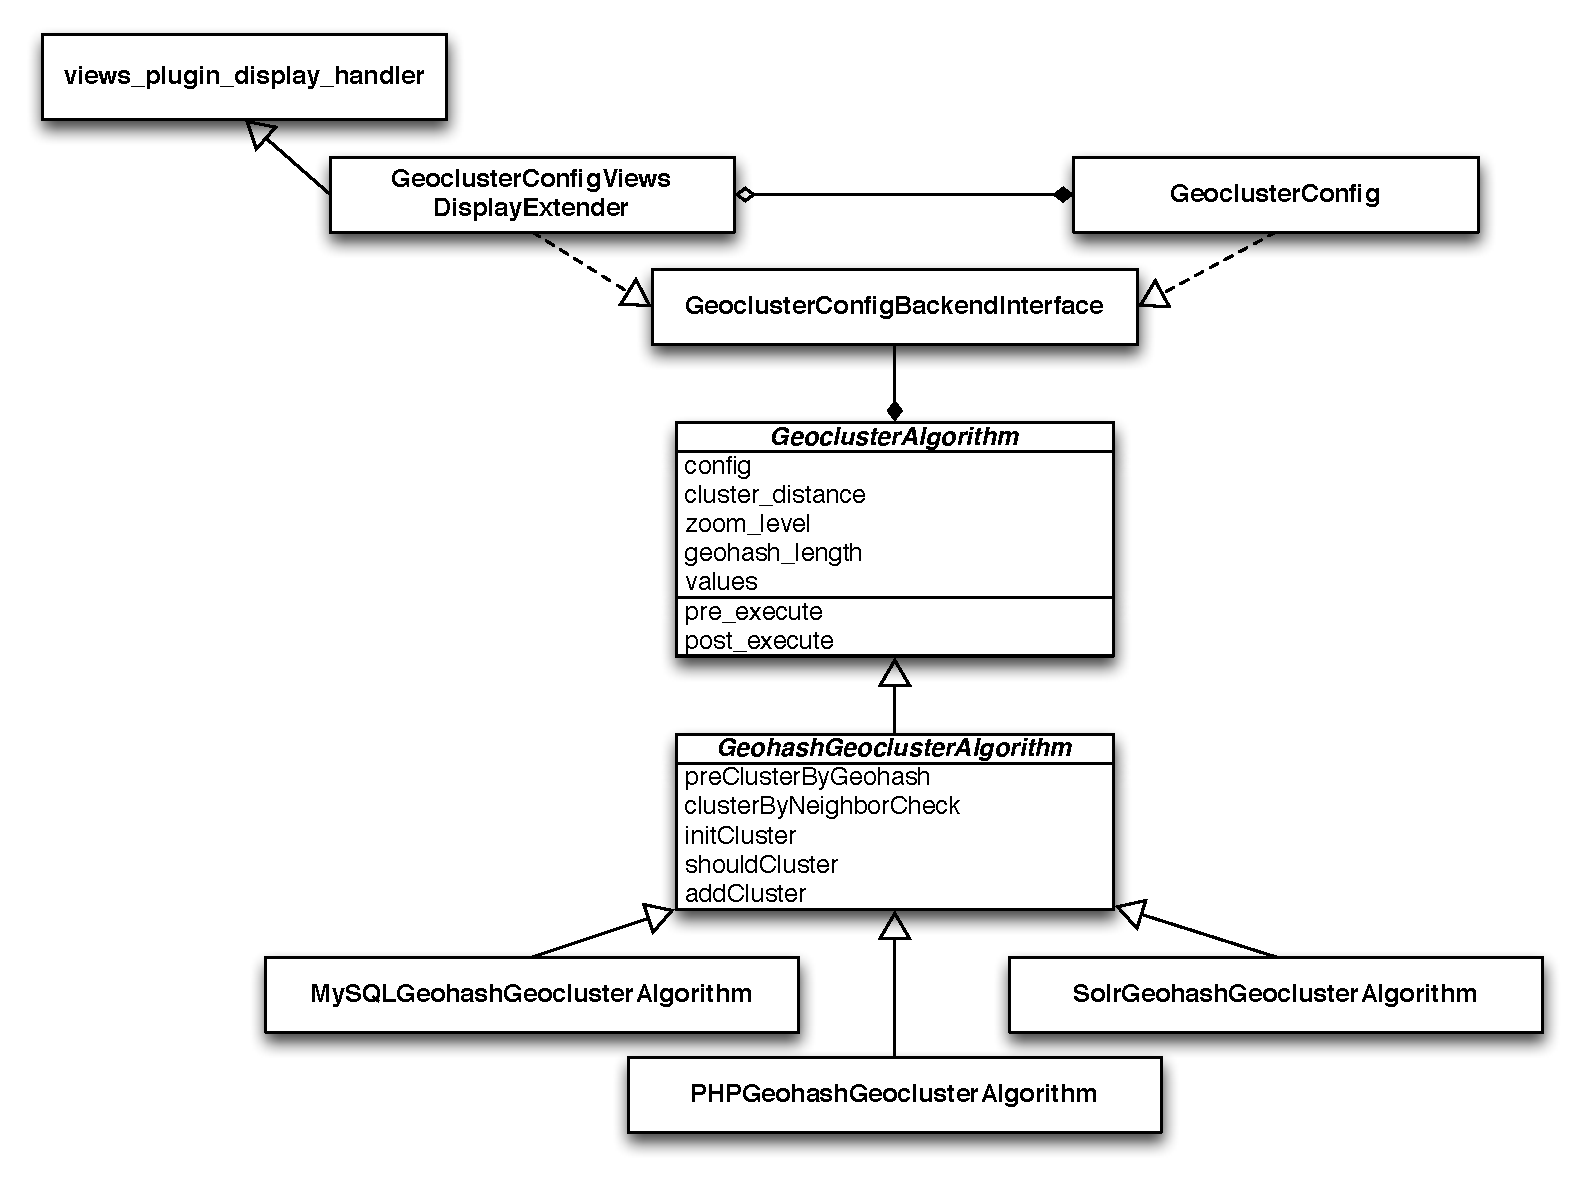
\includegraphics[width=1\textwidth]{figures/geocluster_class_diagram.pdf}
    \caption{Geocluster class diagram.}
    \label{fig:geocluster-class-diagram}
  \end{center}
\end{figure}

Figure \ref{fig:geocluster-class-diagram} illustrates how the \textit{GeoclusterAlgorithm} allows for different variations of the clustering algorithm to be implemented and how the configuration integrates with the Views module. 

\subsection{Configuration of the clustering process}

The Geocluster algorithm depends on three inputs: the data points to cluster, the current zoom level and the minimum cluster distance. The zoom level is passed by the bounding box strategy as a request parameter. In order to configure the rest of the inputs required by the algorithm, a user interface for configuration of the clustering process has been created using the Views plugin system.

When configuring a View, the user may enable Geocluster using a checkbox as illustrated in figure \ref{fig:geocluster-configuration}. If enabled, an additional option set for the clustering process will be displayed.

\begin{itemize}

\item The \textbf{Clustering algorithm} option allows the user to select one of the provided clustering algorithms.

\item The \textbf{Cluster field} option determines the Geofield which should be used as spatial data source for the clustering process. 

\item The \textbf{Cluster distance} option specifies the minimum distance between clusters for the algorithm.

\end{itemize}

\begin{figure}[h]
  \begin{center}
    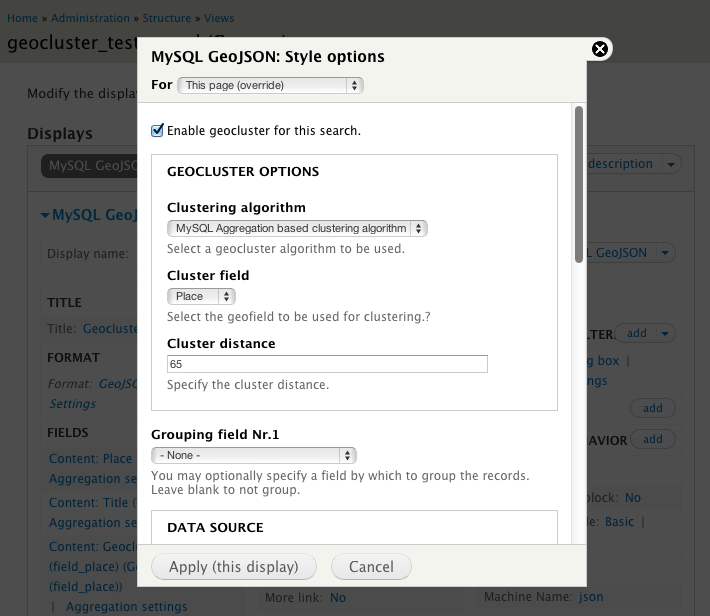
\includegraphics[width=1\textwidth]{figures/geocluster_configuration.png}
    \caption{Geocluster configuration options within the Views administration interface.}
    \label{fig:geocluster-configuration}
  \end{center}
\end{figure}

As indicated by figure \ref{fig:geocluster-class-diagram}, the \textit{GeoclusterConfigViewsDisplayExtender} class integrates the configuration options as a Views plugin. The actual configuration options have been decoupled from the Views-dependent plugin as the \textit{GeoclusterConfig} class. The interface \textit{GeoclusterConfigBackendInterface} abstracts the communication between the configuration classes and the \textit{GeoclusterAlgorithm}. 

\subsection{Implementation of the clustering algorithm}


Three variations of the Geohash-based algorithm have been implemented for Drupal 7. In a first iteration, a \textit{PHP-based} implementation of the clustering algorithm was prototyped to figure out the integration of the algorithm into the Drupal mapping stack. In a second and third iteration, \textit{MySQL-aggregation-based} and \textit{Solr-based} algorithm implementations were added to improve performance support additional use cases. 

\subsection{Integration of the clustering process with Views}





\begin{figure}[h]
  \begin{center}
    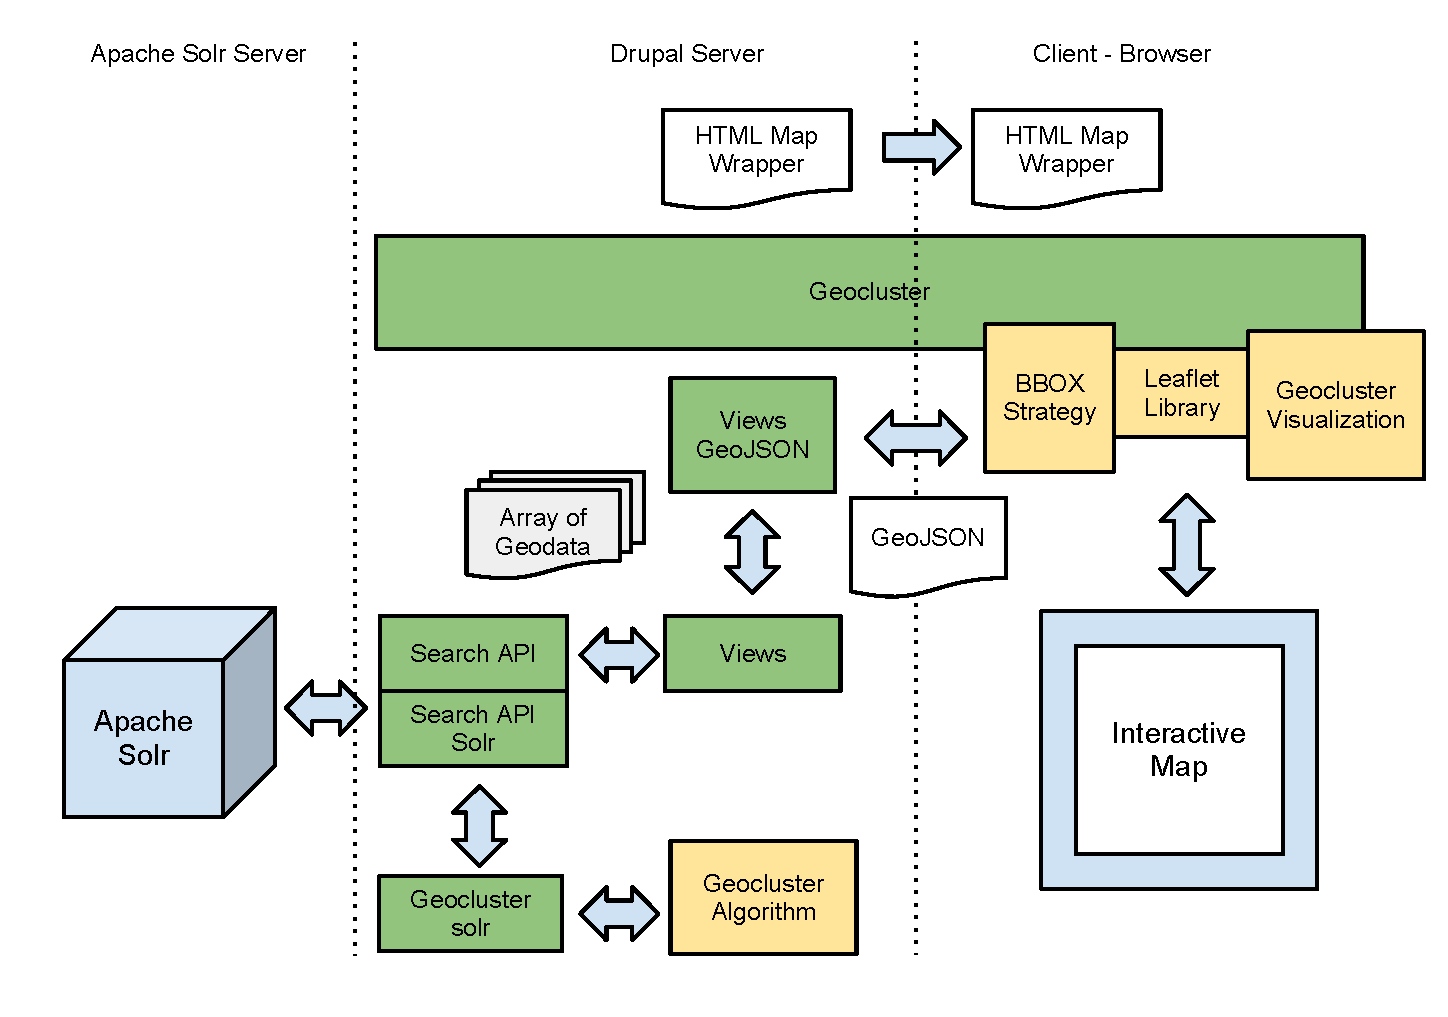
\includegraphics[width=1\textwidth]{figures/geocluster_solr_architecture.pdf}
    \caption{The Drupal Geofield module and related geo data input and storage modules.}
    \label{fig:geofield}
  \end{center}
\end{figure}
